\section{\Sys Design}
\label{sec:catena:design}

At a high level, \Sys makes equivocation about a log statement as hard as double spending a Bitcoin transaction output.
The key idea behind \Sys is to embed statements in Bitcoin transactions and have each transaction spend the previous one.
This is a simple but powerful idea because \emph{it forces the log server to double spend a transaction output if it wants to equivocate}, which is notoriously difficult in Bitcoin.
Thus, \Sys can offer a strong guarantee to clients that they have not been equivocated to.

\Sys operates very simply, as illustrated in \figref{fig:catena-overview}.
The \Sys log server creates a log by issuing an initial transaction called the \emph{genesis transaction}.
The server issues the first statement in the log by creating a new transaction that spends the genesis transaction and commits that first statement via an \opret transaction output (see \secref{sec:background:bitcoin:opret}).
Finally, the server can append new statements to the log by  creating a new transaction that spends the previously-created transaction and commits a new statement.

\Sys clients first obtain the log's genesis transaction, which can be shipped with the higher-level application that \Sys secures (see \secref{sec:model:threat:log-server}).
Then, clients obtain and verify all Bitcoin block headers from the header relay network (discussed in \secref{sec:catena:design:header-relay}).
Finally, clients can ask the \Sys log server for the statements and verify them against the genesis transaction and the Bitcoin block headers.
Importantly, because \Sys transactions are ``chained'' (see \figref{fig:non-equivocation}) and Bitcoin prevents double spends, clients are assured the server has not equivocated (see \secref{sec:model:goals:noneq}).

\Sys's overhead is small.
For each 32-byte statement, the server sends over a 235-byte \Sys transaction and a Merkle path of up to 350 bytes proving that the statement is part of the log.
That amounts to around 600 bytes per statement plus the overhead of downloading all block headers (currently \headerssize), making \Sys very cheap in terms of bandwidth.

% Avg # of TXs is 2000 nowadays. Each proof is 256 bits * log_2(2048) = 256 bits * 11 = 352 bytes. 
% https://blockchain.info/charts/n-transactions-per-block?timespan=all 
%
% Each OP_RETURN TX with a 32-byte payload is 235 bytes => Proof + TX = 235 + 352 =~ 600 bytes
% https://tradeblock.com/bitcoin/tx/8bae12b5f4c088d940733dcd1455efc6a3a69cf9340e17a981286d3778615684 (not sure why this is >250 bytes)
% https://blockchain.info/tx/29c108fbbf672fac9536aa25ae7f3931c9588a0e10650c73ff5883531af2ef45?show_adv=true (235 bytes as expected)
% https://tradeblock.com/blog/analysis-of-bitcoin-transaction-size-trends (average block is around 2000 TXNs)


\subsection{Transaction Format}

\subsubsection{Genesis transaction}
\label{sec:catena:design:genesis}
\Sys logs are identified by a genesis transaction.
This is the first transaction created by the log server when it starts the log.
The genesis transaction effectively acts as the log's ``\pk'': once a client has the log's genesis transaction, that client can verify log updates against it and prevent equivocation.
As discussed in \secref{sec:model:threat:log-server}, a ``\pk'' such as the genesis transaction is a necessary element of any system which aims to prevent equivocation.

\subsubsection{\Sys transactions}
\label{sec:catena:design:transactions}
A \Sys log is just a chain of specially-crafted Bitcoin transactions called \emph{\Sys transactions} (see \figref{fig:catena-overview}).
Our transaction format is simple.
First, a \Sys transaction has one input, which spends the previous \Sys transaction in the chain, and extra inputs for ``re-funding'' the log (see \secref{sec:catena:design:refund}).
Second, a \Sys transaction has two outputs.
The first output is an unspendable \opret output, which commits the log statement, and the second output is a \emph{continuation output}, which is spent by the next \Sys transaction's input.
The genesis transaction also has the same \Sys transaction format.

% or t for top, b for bottom, h for here (https://tex.stackexchange.com/questions/35125/how-to-use-the-placement-options-t-h-with-figures)
\begin{figure}[t]
	\centering
	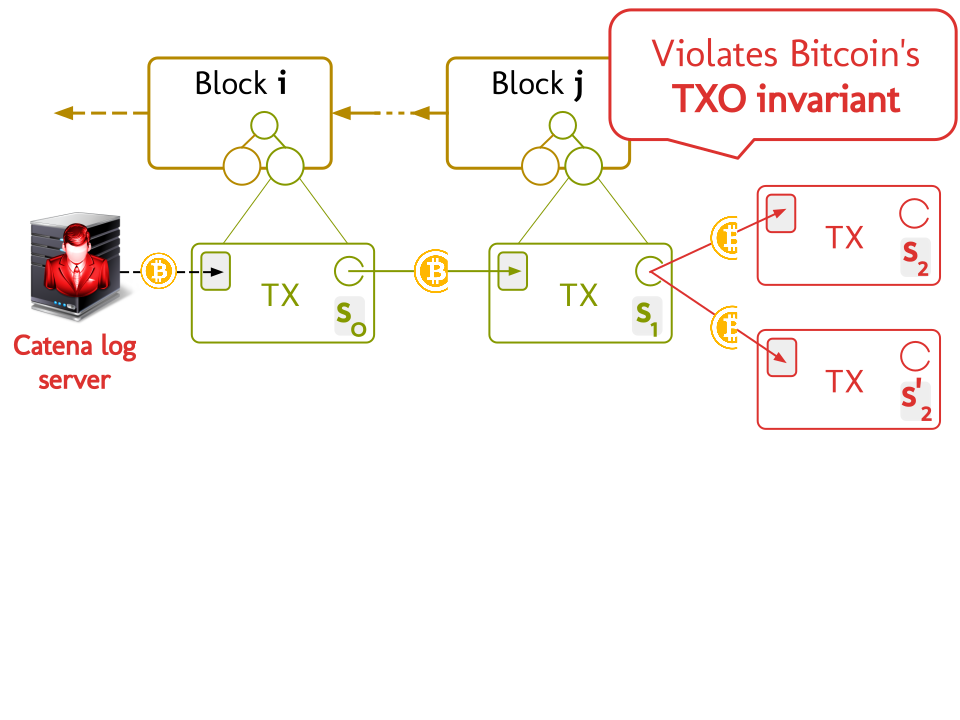
\includegraphics[width=1\columnwidth]{figs/non-equiv.pdf}
	\vspace{-3.2cm}
	\caption{Equivocating in a \Sys log is as hard as double spending in Bitcoin, which requires forking the blockchain (see \secref{sec:background:bitcoin}). This is because \Sys's design requires a new \Sys transaction to spend the previous one, which linearizes the history of statements embedded in those transactions.}
	\label{fig:non-equivocation}
\end{figure}

% Transaction format prevents equivocation
% ----------------------------------------
Our transaction format leverages the fact that Bitcoin miners prevent double spends which, in turn, allows us to prevent equivocation about statements (see \figref{fig:non-equivocation}).
The key idea is that a \Sys transaction has a single spendable output, which means Bitcoin miners will ensure \emph{only a single future transaction spends that output} (see TXO invariant in \secref{sec:background:bitcoin:transactions}).
Thus, a \Sys transaction can only be followed by another \emph{unique} \Sys transaction, which allows us to create a linear history of statements that all \Sys clients can agree on.

% Statement key
% -------------
\Sys transactions just transfer coins from the \Sys log server back to itself, committing log statements and paying fees to Bitcoin miners in the process.
Recall from \secref{sec:background:bitcoin:transactions} that a transaction output specifies a coin amount and a public key that ``locks'' those coins (\ie is authorized to spend them later).
In \Sys, all transaction outputs are locked by the same key called the \emph{statement key}, which is managed by the log server.
This key signs all \Sys transactions, including the statements embedded in them, authorizing the transfer of coins back to the server.
\Sys clients can easily obtain the statement key from the genesis transaction since it is specified in its continuation output.
% (In practice, they obtain the key's fingeprint/address from the genesis transaction's continuation output and the actual PK from the next TXN's input.)
The server can change the statement key in future transactions and clients can easily pick up the new key, but for simplicity we assume it remains the same across all \Sys transactions.

% Transaction fees
% ----------------
As mentioned before, the log server has to pay fees to Bitcoin miners to get its transactions included in the blockchain.
We describe how this works in \secref{sec:catena:design:refund} and we analyze the server's cost per \Sys statement in \secref{sec:prototype:fees}.


\subsection{Header Relay Network}
\label{sec:catena:design:header-relay}
We want to avoid stressing Bitcoin's P2P network, which has a limited connection capacity that would be quickly depleted by \Sys clients.
There are currently around 5500 full Bitcoin nodes, each by default capable of handling up to 117 incoming connections\cite{bitcoin-bitnodes-21co,bitcoin-p2p}.
Thus, Bitcoin's P2P network currently supports at most 643,500 incoming connections at a single point in time, some of which are already used up by Bitcoin thin clients for user wallets.
Importantly, these connections need to be long-lived so as to allow \Sys clients to discover and connect to a diverse set of Bitcoin peers.
As a result, if each \Sys client were to maintain 8 outgoing connections to Bitcoin's P2P network, then \Sys would not scale beyond tens of thousands of clients without putting significant stress on the Bitcoin network.

To provide scalability, we propose using a header relay network (HRN) that is well connected to the Bitcoin P2P network and can serve block headers to hundreds of thousands of \Sys clients.
An HRN node operates as a full node in the Bitcoin P2P network, contributing to its health while providing an interface to \Sys clients for obtaining block headers fast.
However, note that HRN nodes do not mine nor attempt to reach consensus on block headers: they just gossip and verify blocks like the rest of the Bitcoin P2P network.
\Sys clients trust the HRN to serve them with the latest Bitcoin block headers.
Importantly, clients ask multiple HRN nodes for block headers to ensure they are not being eclipsed by a single malicious HRN node.
We discuss attacks on the HRN in \secref{sec:attacks:hrn}.

% Boootstrapping HRNs
% -------------------
A header relay network can be bootstrapped in various ways.
The simplest way is to have a set of volunteer HRN nodes that act as an extension of the Bitcoin P2P network.
Another way is to rely on current blockchain explorers\cite{bitcoin-blockchaindotinfo, bitcoin-blockexplorerdotcom, bitcoin-blockrdotio,bitcoin-blocktraildotcom} since they are well connected to the Bitcoin network and already provide public APIs for fetching block headers.
A diverse HRN could be implemented by publishing block headers across various websites, such as Twitter, Facebook or GitHub, in a publicly-verifiable manner similar to how Keybase\cite{keybase} users publish identity proofs.
A peer-to-peer HRN can be bootstrapped amongst \Sys clients themselves.
\Sys clients can occasionally fetch block headers from the Bitcoin P2P network and then distribute them amongst themselves.
To avoid stressing Bitcoin P2P nodes, each client would query the Bitcoin P2P network with probability inversely proportional to the size of HRN (estimated using known techniques\cite{p2p-size-estimation}).
Finally, Sybil attacks\cite{sybil} in all these types of HRNs can be addressed by requiring HRN nodes to ``burn'' bitcoins in a publicly-verifiable manner (see \secref{sec:background:bitcoin:opret}) and tie their identity to those burned coins.

% https://bitcoin.stackexchange.com/questions/37344/is-the-spv-client-model-scalable
% At best, if a full node can read blocks at 20MB/s from disk and filter them with close to no overhead, it would only be able to send 20 filtered blocks per second.
% With 5500 nodes in the network, in an ideal world, this would amount to a total available bandwidth of 110,000 filtered blocks per second.
% However, a full node's throughput in terms of block headers/sec is quite high: easily serve 100,000 headers/sec to a single client and more to multiple clients.
% \Sys nodes add close to no overhead to Bitcoin nodes, requiring little time to sync up: a few seconds for downloading \headerssize of block headers.


\subsection{Auditing a \Sys Log}
\label{sec:catena:design:auditing}
% Overview of auditing
% ---------------------
To audit a log, clients download the \Sys transaction chain and verify that transactions are signed and spend each other correctly using the statement key.
Clients first download and verify block headers from the header relay network and then download and verify \Sys transactions and their Merkle proofs from the log server.
This way, \Sys clients avoid Bloom filtering on Bitcoin's P2P network, which causes significant disk activity for full nodes (see \secref{sec:background:bitcoin:thin}).
Finally, auditing is cheap for \Sys clients as they only download small transactions and Merkle proofs (600 bytes) and not full Bitcoin blocks (1 MB).

% Verifying a transaction
% -----------------------
To verify a new \Sys transaction $tx_i$, a client checks that:
\begin{enumerate}
\item $tx_i$ is in the correct \Sys format.
\item $tx_i$ is correctly included in a Bitcoin block with a Merkle membership proof.
\item The first input of $tx_i$ spends the continuation output of the previous \Sys transaction $tx_{i-1}$.
\item $tx_i$ is signed correctly with the statement key of the log.
\item $tx_i$ has a sufficient number of confirmations (we recommend at least 6).
\end{enumerate}

% Checking transaction signatures
% -------------------------------
It's important to understand that without clients verifying transaction chaining (\ie step 3 and 4 above), a malicious log server can equivocate about statements in the log.
For example, consider two \Sys clients $c_1$ and $c_2$ which correctly obtain the genesis transaction $\txgen$ of the log but do not verify transactions are chained.
In this attack, the malicious log server issues two \Sys transactions that commit two different statements $s_1$ and $s_1'$ respectively but, importantly,  \emph{do not spend} the genesis transaction.
Instead they spend some other transactions and get included in the blockchain.
The attack is straightforward: the log server shows client $c_1$ the transaction for $s_1$ but hides the one for $s_1'$.
Similarly, it shows client $c_2$ the transaction for $s_1'$ and hides the one for $s_1$.
As a result, the log server can easily equivocate to clients who don't verify transaction chaining as they cannot ensure the server is not hiding an inconsistent statement.
To conclude, in \Sys, clients prevent this attack by checking that every statement they accept is part of a transaction that spends the previous transaction's continuation output, chaining all the way back to the genesis transaction.


\subsection{Blockchain Reorganizations}
\label{sec:catena:design:reorgs}
Like Bitcoin, \Sys also needs to deal with small day-to-day accidental forks or \emph{blockchain reorganizations} (see \secref{sec:background:bitcoin:consensus}).
These small forks are automatically resolved by the Bitcoin network: as more blocks are found, eventually one of the forks overtakes the other one and becomes the main chain\cite{blockchainproto}.
To be certain payments are not reversed by these small reorganizations, Bitcoin merchants only consider a block and its transactions confirmed if 6 or more blocks are built on top of it.

\Sys also allows clients to set their own application-specific number of required confirmations before accepting a statement (a minimum of 6 is recommended).
As a result, \Sys makes a trade-off between resilience to forks and latency of accepting statements.
Additionally, as a security measure against longer accidental forks, \Sys clients remember recently-issued statements.
This way, if a statement is withdrawn due to a reorganization, \Sys clients can ensure the reissued statement matches the previously seen one.


\subsection{Paying for a \Sys Log}
\label{sec:catena:design:refund}
A \Sys log server must pay Bitcoin transaction fees to start a log and append statements to it.
Initially, the \Sys log server must obtain some bitcoins (BTC), perhaps from a Bitcoin exchange\cite{bitcoin-exchanges}.
Then, the server can issue the log's genesis transaction and pay for its fee.
The server locks some coins in the genesis transaction's continuation output which can ``fund'' future log transactions.
To issue the first statement, the server signs a new \Sys transaction with the statement key.
This transaction commits the statement (via an \opret output), transfers the genesis transaction's coins back to the log server and leaves a small fee for the miners.
As before, the remaining coins are locked in this new transaction's continuation output.
The server repeats this process for every new statement, spending the coins locked in the previous \Sys transaction, until it runs out of funds.
We analyze the costs of running a \Sys log in terms of transaction fees in \secref{sec:prototype:fees}.

% or t for top, b for bottom, h for here (https://tex.stackexchange.com/questions/35125/how-to-use-the-placement-options-t-h-with-figures)
\begin{figure}[t]
	\centering
	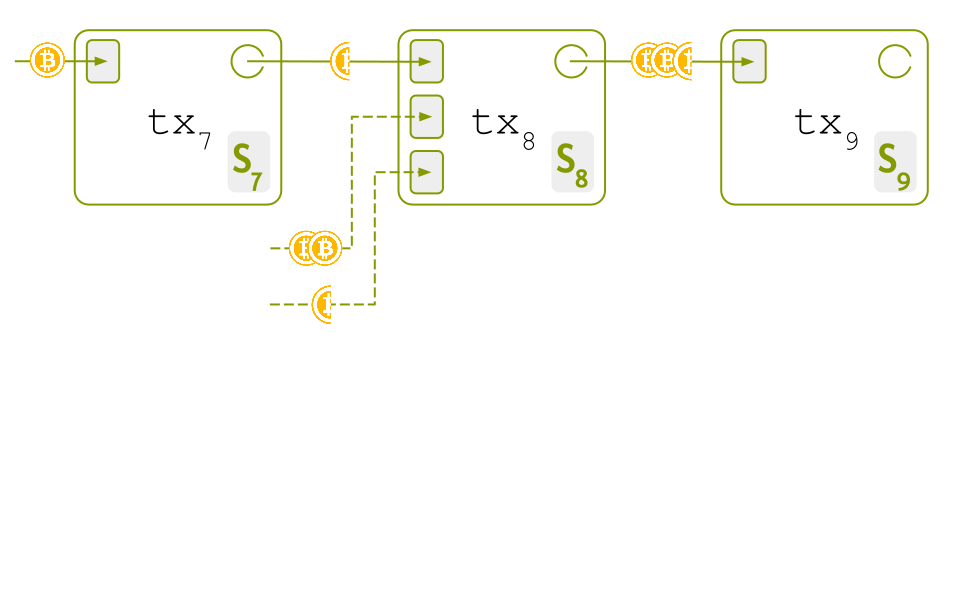
\includegraphics[width=1\columnwidth]{figs/refunding.pdf}
	\vspace{-3.1cm}
	\caption{A \Sys chain can be ``re-funded'' by allowing the next transaction in the chain to have additional inputs that lock extra coins in that transaction's continuation output. In this example, \Sys transactions pay .5 BTC as a fee so to ensure $tx_8$ does not run out of coins we ``re-fund'' it using extra inputs.}
	\label{fig:refunding}
\end{figure}

To ``re-fund'' the chain, \Sys transactions can have additional inputs that lock extra coins in that transaction's continuation output (see \figref{fig:refunding}).
Importantly, these inputs can only be used to add extra funds and cannot be used to maliciously join two different logs.
This is because we restrict \Sys transactions to only use their first input to spend a previous \Sys transaction.
Thus, clients can easily detect if a \Sys transaction tries to point to two distinct previous \Sys transactions by using additional inputs.